\documentclass[conference]{IEEEtran}
\IEEEoverridecommandlockouts
% The preceding line is only needed to identify funding in the first footnote. If that is unneeded, please comment it out.
\usepackage{cite}
\usepackage{amsmath,amssymb,amsfonts}
\usepackage{algorithmic}
\usepackage{graphicx}
\usepackage{textcomp}
\usepackage{xcolor}
\makeatletter
\newcommand{\linebreakand}{%
  \end{@IEEEauthorhalign}
  \hfill\mbox{}\par
  \mbox{}\hfill
  \begin{@IEEEauthorhalign}
}
\makeatother

\def\BibTeX{{\rm B\kern-.05em{\sc i\kern-.025em b}\kern-.08em
    T\kern-.1667em\lower.7ex\hbox{E}\kern-.125emX}}
\begin{document}

\title{A Low-Cost Two-Tier Emergency \\
Communication System\\
}
\author{\IEEEauthorblockN{Anek Sreedhar T S}
\IEEEauthorblockA{\textit{School of Electronics Engineering} \\
\textit{Vellore Institute of Technology, Chennai Campus}\\
Chennai, India \\
aneksreedhar@gmail.com
\\ORCID: 0009-0001-0070-5743}
\and
\IEEEauthorblockN{Avinash Nair}
\IEEEauthorblockA{\textit{School of Electronics Engineering} \\
\textit{Vellore Institute of Technology, Chennai Campus}\\
Chennai, India \\
avinash.nair2004@gmail.com
\\ORCID: 0009-0002-7956-6412}
\linebreakand % This command creates the line break for the 2x2 format
\IEEEauthorblockN{Dasangam Akash}
\IEEEauthorblockA{\textit{School of Electronics Engineering} \\
\textit{Vellore Institute of Technology, Chennai Campus}\\
Chennai, India \\
dasangamakash515@gmail.com
\\ORCID: 0009-0006-3714-3875}
\and
\IEEEauthorblockN{Usha Kiran Kommuri}
\IEEEauthorblockA{\textit{School of Electronics Engineering} \\
\textit{Vellore Institute of Technology, Chennai Campus}\\
Chennai, India \\
usha.kiran@vit.ac.in
\\ORCID: 0000-0002-5651-1374}
}
\maketitle

\begin{abstract}
When a natural disaster strikes in developing countries such as India, there is an entirely predictable and catastrophic failure of the communication infrastructure due to its centralized infrastructure, which in turn terminates the connection between the authorities and the citizens. This paper goes into depth about the current state of emergency infrastructure and addresses the gaps in their decentralized and infrastructure-independent nature by proposing an inexpensive, two-tier hierarchical Lora mesh network. This system operates on the 433MHz ISM band, which is license free. It consists of cheap portable civilian nodes and an authorized base station node for the authorities; the latter utilizes a QFH (Quadrifilar Helical Antenna), used for its hemispherical radiation pattern. The QFH antenna design is simulated in CST studio to achieve capacitive loading for reduced resonant height. The network interface is built upon the open source, Meshtastic project which allows for fully mature protocols along with state of the art encryption, AES-GCM. The work is successful in validating the theoretical framework laid for this architecture and proves its efficiency in such disaster scenarios.
\end{abstract}

\begin{IEEEkeywords}
component, formatting, style, styling, insert
\end{IEEEkeywords}

\section{INTRODUCTION}
% \begin{figure}[htbp]
% \centerline{\includegraphics[width=\columnwidth]{figures/fig1.png}}
% \caption{Cell Tower Collapsed Due to Hurricane}
% \label{fig}
% \end{figure}

In developing countries like India, natural disasters pose a way bigger problem compared to other countries. This is due to the systemic and catastrophic failure of the centralized communication infrastructure. This has been a recurrent issue, in Orissa Super Cyclone (1999), the Bhuj Earthquake (2001) and the Kerala Floods (2018). The underlying problem is not just the disaster but also the centralized highly interdependent nature of network infrastructure, if power grid or the cell tower or internet fiber poles is damaged, the system goes down. Hence, there are multiple points of complete failure. 

This failure is mostly predictable when a disaster strikes. It cuts off the very needed communication channel between the citizens and the authorities, causing more casualties during these tumultuous times. Hence, there is a need for decentralized infrastructure-independent architecture which allows a hierarchical mode of communication between the authorities and citizens, allowing the authority to broadcast information like aid and food available at a nearby location and receive messages from citizens, like road-blocking or building collapse.  

Here we discuss such a system architecture built upon much foundational research, but building upon their gaps. This makes it robust, redundant, delay tolerant and relatively inexpensive, allowing easier and cheap dissemination of the citizen units. 

The mesh algorithm provides a highly redundant, store and forward network with confidentiality and authenticity preserved during communication.

\section{LITERATURE REVIEW}

A review of some of the initial and more recent work [1-15] on the use of LoRa devices for emergency messaging shows some good ideas, but they are scattered about. Wang et al [15] divide the systems into three classes for the improvements available today, satellite, cellular, and home-made. If the central stations are disturbed, then the satellite systems and cell systems fail; but there is good promise for peer to peer LoRa communications. However, when we examine more carefully the ways used to employ the LoRa technology we find a lack of development, in that no over-all system has been given to combine the improvements in five separate and important fields, organization of the network, signaling systems employed, means used for executing the code, means for protecting the system, and methods for communicating with the signal transmitter. 

A very large part of the present problem is in the field of wireless network systems. In the majority of the works, there is a great dependence on one of two unsuccessful systems. One is a very heavy dependence on central stations supplied with costly and difficult to manage remote systems, such as LoRaWAN. This may be seen in the system of Douklias et al [11], the system of Dubey et al [4], or the signal detection system of Bouras et al [9]. These works have in common systems for transmitting messages, using relay stations and communicating them through links in the network, such as the 4G systems, or satellites, but they thus have one great defect, namely that the very defect from which the plan the central organization suffers when a disturbance occurs. In answer to this another form of network systems has appeared, these give decentralized, homogeneous, P2P meshes. Their use may be seen in the DisasChat system of Dutta et al [1], and MauMe of Mari and Gabillon [10], and Muladi’s system of the Meshtastic tracker [12], which show that they are systems which make it easily possible of providing adequate communication without the necessity of the use of a central station. There are however disadvantages. To be a homogenous system, it must depend upon the use of the same sort of low power devices by the users, and in consequence a restriction in the usable distance and distance of control. Some systems have tried hierarchical systems, but, as has been shown, they have for the most part turned out to be too cumbersome and too greedy of power, such as the system utilizing AI of Todakar et al [2], or they are used in great part for some sole use, and are one-way transmission systems as observed in the case of the earthquake warning system of Ranasinghe et al [8]. This separation creates a hole - a viable two- or more way layer structure that can connect ordinary people directly with the command centers through the combination of the strong mesh oriented survivorship skills with the strong range hubs. 

This effect is made worse due to the weak features of the protocol sets about how to code means of communication or run a program or provide safety. The overt failure in the area of a chain form of signal structure shows up in the form of a communication saturation through too many cycles of the general loop of messages which can lead till disaster therefrom results when everything tends to fall dead. Some of the savants can get over it by means of large structure employed, working over the habit, as Schmidt's bande BPoL/DTN7 method [3] shows or the rf95modem experimental work of Höcht [13] or. The brands do not mostly lend themselves to the kind of abc general type of communication desirable in parts of minutes following a catastrophe disaster; but varieties are progressed which can communicate in rapid flow of information, as the MauMe process of spreading communications naturally of mornings development of study Mare and Gabillon's [10] which of itself needs the ACK or passage of reply signal in factor about the which coincidence messages are given on recognised paths of communications to give such communication flow filling the approach to communication space. 

These lead to being operating in their density of paths and productive capability to the fining up of channel and double despatch of messages wherever connecting about recognized wave lengths over links to centers, these of ways have their dacile habitation and ment of freely running new lines of patches to carry near by freight of what to do next, which is displaced in the method of quite another means of sending of messages without expense of memory in the operation of being brief recollections, it is known that the common, simple and somewhat abrupt, but well intentioned method of spreading the messages without the memory factor can be sent along, this complicatory machinery to shift into with numbers, but render that due feature useful intervening in the real problems of coding and systems by processes as are introduced in the tools of Meshtastic, giving methods of analytic degree of work on the working of the conception given by the notion of Mulidai et al. [12] are running on ready made circuit range in their operations as standard forms out of box. The conversion to a flouring function on the cheap varieties by being placed on the broad framework of the cheaper ESP32-WROOM-32 chips requires far more hands or producing effort than is it in itself to work out handled on experiment, but on its approach wild active channels bring space allowances for cheap production variety of formations or phrasing results. Curiously safety is believed not to work out in the manufacture of formations till it is too late.. Plenty of setups - like 2, 3, 4, 6, 7, 8, 9, 11, 12, and 15 - barely bring it up at all. When they do touch on it, some openly skip protection, sending data raw [10], while others just don’t finish the job. The best attempt spotted so far, DisasChat [1], uses AES-256 to hide info yet misses built-in checks for tampering or source trust. Not once does anyone use a full AEAD method like AES-GCM, which handles secrecy, validity, and verification together. 

A big issue remains when building antennas for the base station used by the authority. One main problem at lower frequencies - say, 433 MHz - is that a working Quadrifilar Helical Antenna tends to take up too much space. Older studies, like Fusco’s team [14], along with recent ones focused on LoRa, such as Ariessaputra et al. [5], usually try shrinking it by changing how the metal parts are shaped; examples include adding small insulating breaks or tweaking coil patterns. That leaves room for something new: using 3D printing so the support structure itself plays a role in signal handling. Instead of just being a frame, the printed part - maybe made from PLA plastic - could act like a capacitor by affecting electric fields, pushing the tuning frequency down and letting the actual wire loops get smaller - an idea not yet explored. 

Overall, past studies offer useful pieces - but only bits and parts. Not one full setup’s been suggested to fix those five combined shortcomings. Our work introduces a framework stitching together fresh fixes for each of the five areas, building just one solid, real-world-ready emergency messaging system. 

\section{METHODOLOGY}

\subsection{System Architecture and Design} 
\begin{figure}[htbp]
\centerline{\includegraphics[width=\columnwidth]{figures/fig2.png}}
\caption{Block Diagram of the Node (microcontroller with OLED module and RA02 LORA module)}
\label{fig}
\end{figure}
We will explain the architecture of the two parts of this system, the civilian node and the base station node. Both are conceptualized as microcontroller-based nodes, utilizing components such as an ESP32-WROOM-32, an OLED Display (ssd1306), and a LoRa module (RA02) with an antenna.  

\begin{figure}[htbp]
\centerline{\includegraphics[width=\columnwidth]{figures/fig3.png}}
\caption{Fabricated Civilian Node}
\label{fig}
\end{figure}
The difference lies in the kind of antenna they use and how the power is supplied. The civilian node is designed as a portable unit for communication with authorities, utilizing a simple commercially available dipole antenna for transmitting and receiving, and powered by a 18650 lithium battery. 


Meanwhile, the base station node is designed for high-power operation at disaster management authority locations, such as a DEOC (District Emergency Operation Centre), to broadcast and receive disaster-related communication. It is conceptualized as main-powered and equipped with a quadrifilar helical antenna for extended range. 



We have chosen the 433 MHz frequency as this frequency is delicenced for low power devices for the purpose of medical and scientific uses. Our input power is below 15 dBm, making this viable for our need. 

\subsection{Antenna Design and Simulation}

\begin{table}[h!]
\centering
\caption{General parameters}
\label{tab:general_params}
\begin{tabular}{|l|c|}
\hline
\textbf{Parameter (Symbol)} & \textbf{Value (Unit)} \\
\hline
Wavelength ($\lambda$) & 692.8 mm \\
\hline
Compensated wavelength ($\lambda_c$) & 739.9 mm \\
\hline
Bending correction ($b_{corr}$) & 0.8 mm \\
\hline
\end{tabular}
\end{table}

\begin{table}[h!]
\centering
\caption{Larger Loop}
\label{tab:larger_loop}
\begin{tabular}{|l|c|}
\hline
\textbf{Quantity (Symbol)} & \textbf{Value (Unit)} \\
\hline
Total length ($L_1$) & 759.1 mm \\
\hline
Compensated total length ($L_{1c}$) & 762.6 mm \\
\hline
Horizontal separator ($R_1$) & 78.1 mm \\
\hline
Vertical separator ($V_1$) & 303.1 mm \\
\hline
Compensated values ($R_{1c}, V_{1c}$) & 74.1 mm, 299.1 mm \\
\hline
Antenna height ($H_1$) & 177.6 mm \\
\hline
Internal diameter ($D_{i1}$) & 74.1 mm \\
\hline
\end{tabular}
\end{table}

\begin{table}[h!]
\centering
\caption{Smaller Loop}
\label{tab:smaller_loop}
\begin{tabular}{|l|c|}
\hline
\textbf{Quantity (Symbol)} & \textbf{Value (Unit)} \\
\hline
Total length ($L_2$) & 721.4 mm \\
\hline
Compensated total length ($L_{2c}$) & 724.8 mm \\
\hline
Horizontal separator ($R_2$) & 74.3 mm \\
\hline
Vertical separator ($V_2$) & 288.1 mm \\
\hline
Compensated values ($R_{2c}, V_{2c}$) & 70.3 mm, 284.1 mm \\
\hline
Antenna height ($H_2$) & 168.8 mm \\
\hline
Internal diameter ($D_{i2}$) & 70.3 mm \\
\hline
\end{tabular}
\end{table}

The quadrifilar antenna is used here for its circular polarization and hemispherical radiation pattern. We utilized John Coppens’ well-reputed QFH calculator for designing the dimensions of the antenna, which is based on prior foundational work in QFH antenna, like the design shown by George Goodroe (KF4CPJ) [x].  



There are two orthogonal loops involved, one longer than the other, for achieving circular polarization. This removed the need for ground/reflector for back-reflection to increase the directivity. The calculator utilized formulae and look up table from the existing literature. See appendix for those. After calculator dimensions were found we moved on to synthesis.

\begin{figure}[htbp]
\centerline{\includegraphics[width=\columnwidth]{figures/fig4.png}}
\caption{QFH Antenna modelled in CST Studio}
\label{fig}
\end{figure}

Initial antenna dimensions were then simulated in the software CST Studio and the S11 graph checked to verify the resonance at correct frequency and the radiation pattern. But that size was too large for our testing purposes so utilised a capacitive loading method using, dielectric in our case, PLA scaffolding that holds the antenna but also adds capacitance shifting the resonance to lower frequency giving us leeway to shrink the coil length to get back to correct resonant frequency. This is verified by parametric analysis after adding PLA scaffolding. 

% \begin{figure}[htbp]
% \centerline{\includegraphics[width=\columnwidth]{figures/fig5.png}}
% \caption{QFH Antenna constructed}
% \label{fig}
% \end{figure}

 

% \begin{figure}[htbp]
% \centerline{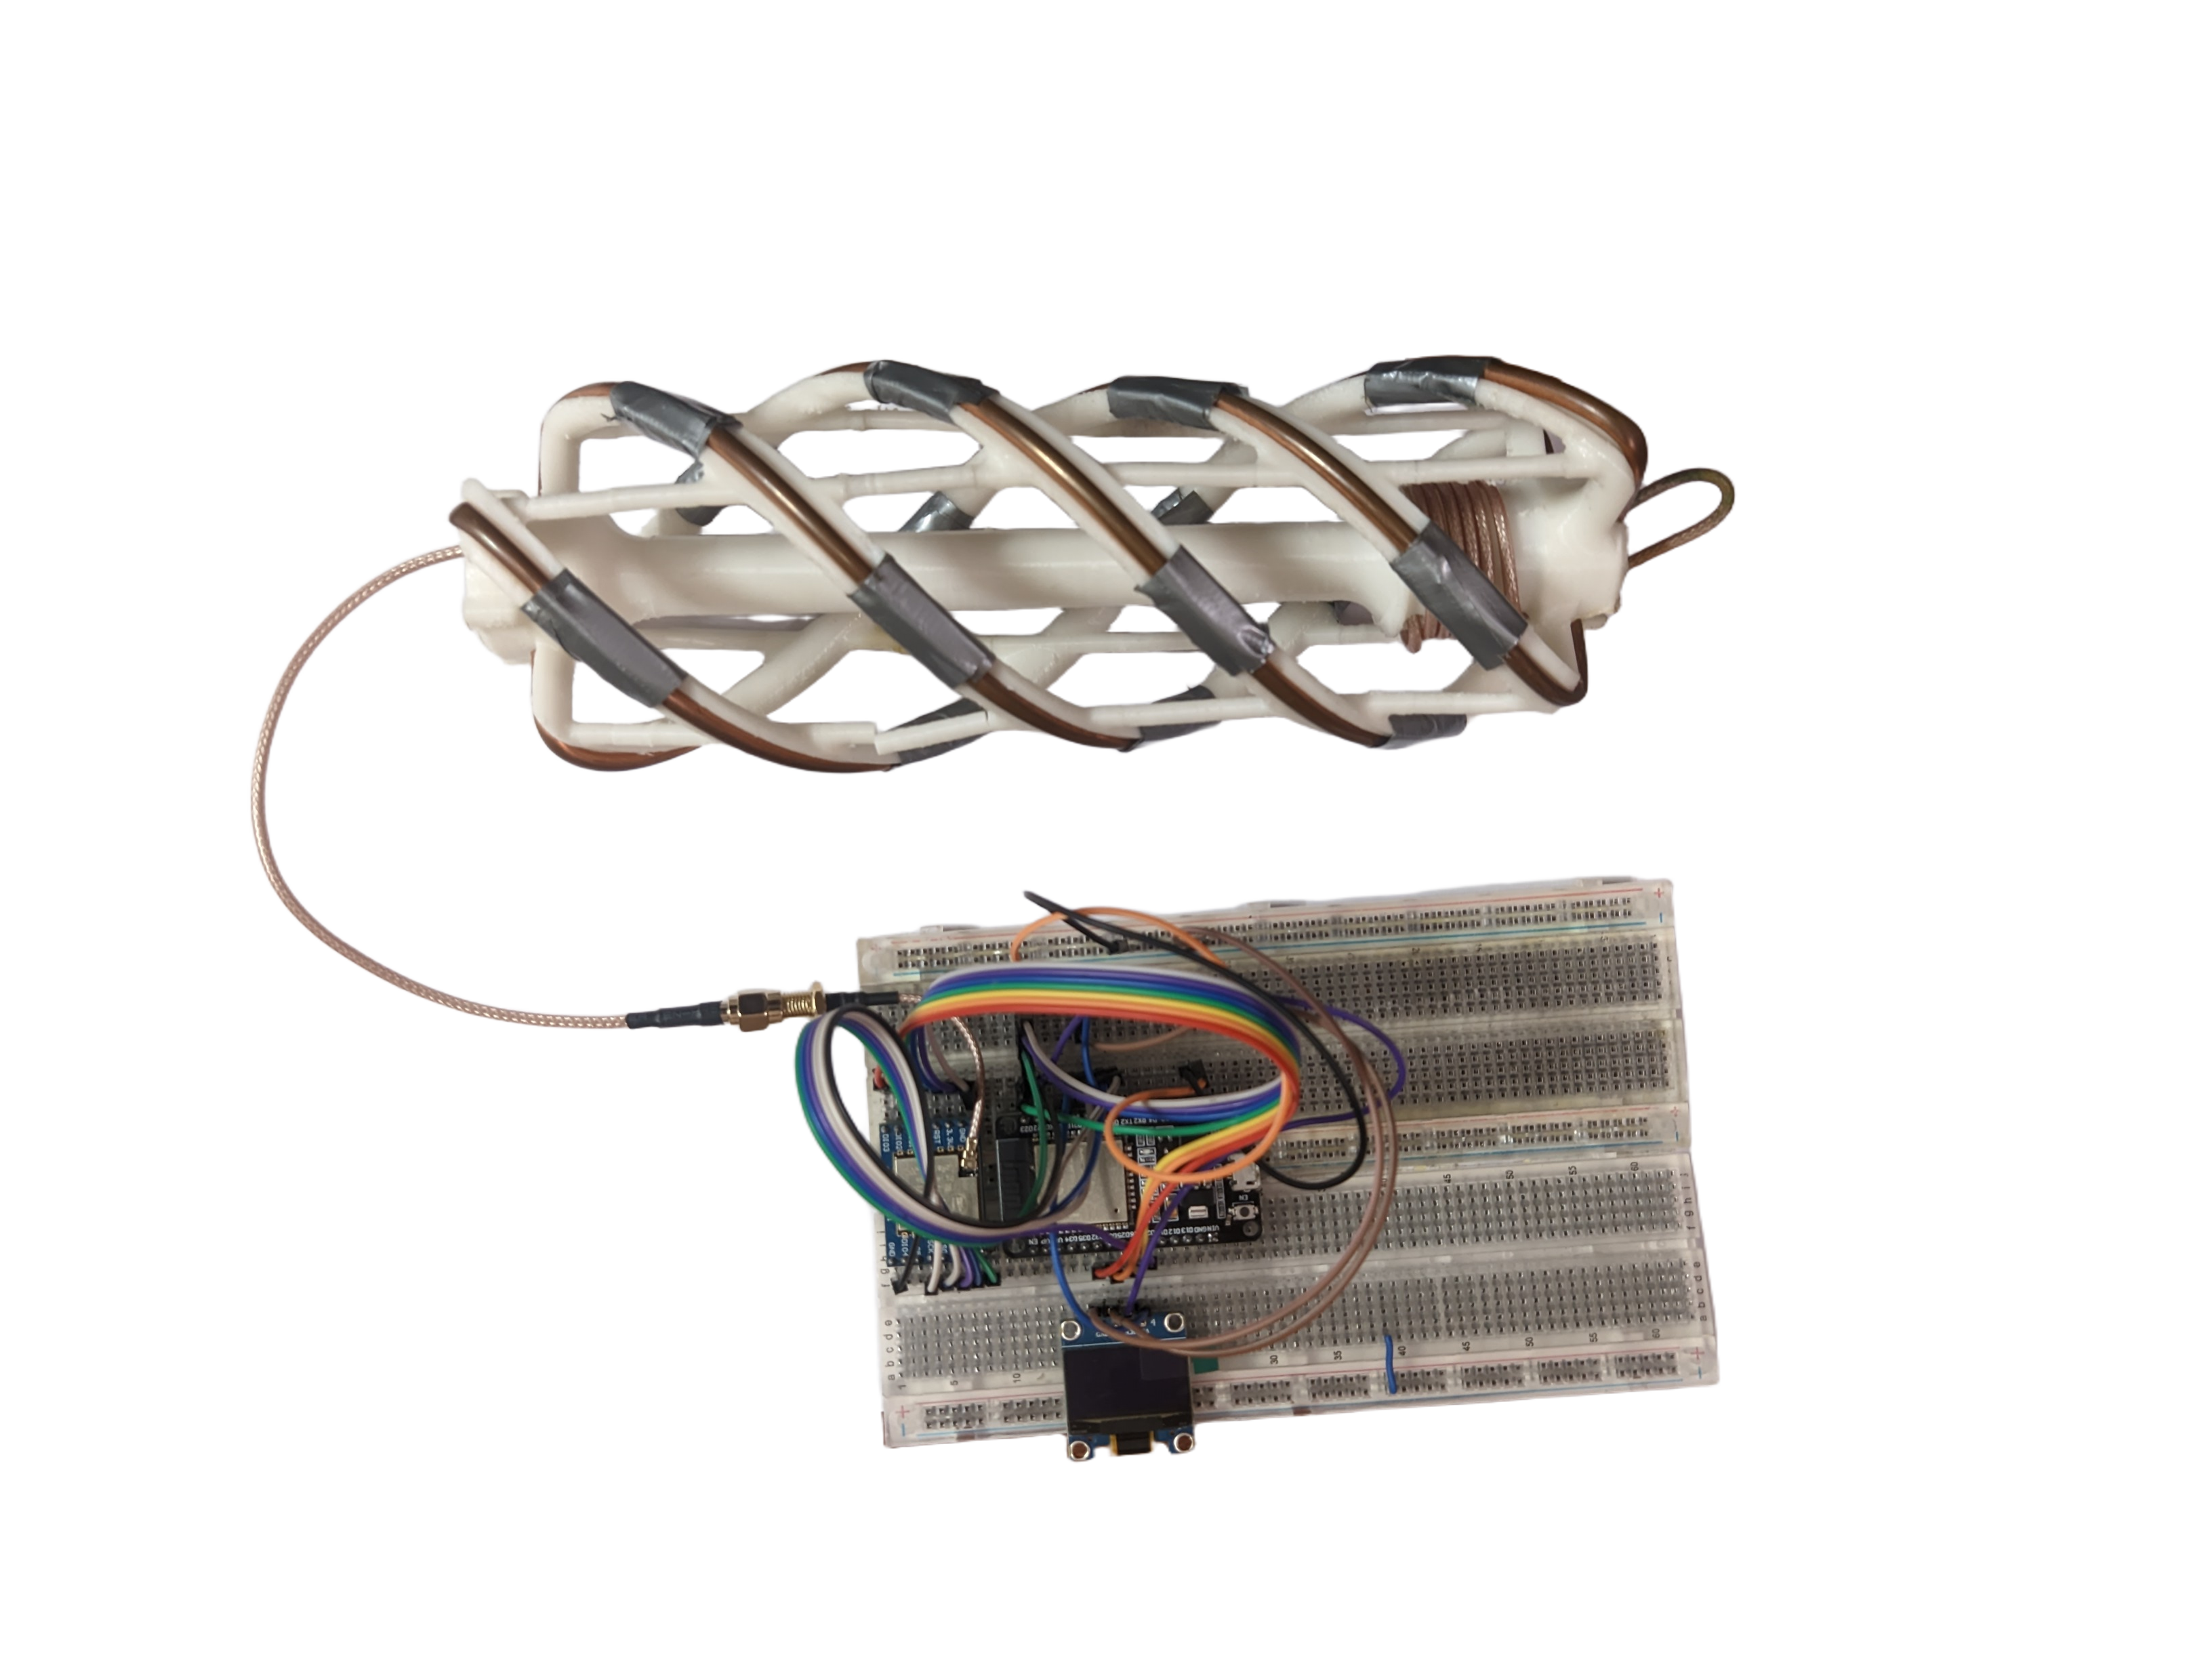
\includegraphics[width=\columnwidth]{figures/fig6.png}}
% \caption{Base Station Node with the QFH antenna}
% \label{fig}
% \end{figure}

\subsection{Network Protocol and Software Implementation}

The code for the system was developed in C++ coding language for its objected oriented paradigm needed for the libraries for we used which included ‘RadioLib’ for LoRa handling and ‘Crypto’ for encryption. The code is derived from the open-source repository for mesh based off-grid LoRa communication, ‘Meshtastic’, but since the project doesn’t support the cheap available, ESP32-WROOM-32, changes were made to many parts of the code. We used PlatformIO IDE to deploy the code. This software stack helped in creating node-to-app communication and the mesh protocol. 

\begin{figure}[htbp]
\centerline{\includegraphics[width=0.6\columnwidth]{figures/fig7.png}}
\caption{Chat Interface of the App}
\label{fig}
\end{figure}
The application interface managed the connection from microcontroller to phone using Bluetooth Low Energy (BLE) and conversion of user messages and mobile GPS data to and from packets in LoRa. 

The transmitted packet contains packet structure, structural information about the packet like Destination, Source and Packet ID along with a Time-to-Live counter which counts hops left to limit packet propagation and the encrypted data. 

For Channel access, we use Carrier-Sense Multiple Access with Collision Avoidance protocol, so before sending any packets, each node performs Channel Activity Detection (CAD). If it detects that channel is busy, it will wait for a random backoff window, with a SNR based varying contention window (CW). 

Along with this procedure, for routing, a flooding-based algorithm is performed, but to prevent the storming issue involved in normal flooding, there is random, short backoff period each node has to adhere to before reading a received packet, if the same packet is received again, that packet gets dropped. 

The encryption used for securing the message is AES-GCM to also achieve integrity and authenticity along with confidentiality as GCM adds the authentication tag which proves lack of alteration while transmission. This especially helps when dealing with decentralized ad-hoc networks like this one. 

\subsection{Network Validation and Simulation}

A multi-stage simulation plan was executed to validate the performance of the individual components and the network. The QFH antenna's performance was validated using CST Studio to verify its S11 (Return Loss) and thereby VSWR to verify its working at the correct frequency.

For network validation, range simulations were conducted to understand propagation relative to power. This approach allowed for testing the mesh algorithm's effectiveness across various scenarios, as the full extent of range performance could be understood through simulation, which incorporated antenna height and power parameters. The mesh nature of the network, including intermediate relaying (e.g., A – B – C structure), was visualized and validated through network simulations.  

\section{RESULTS} 

\subsection{QFH Antenna Simulation}
\begin{figure}[htbp]
\centerline{\includegraphics[width=\columnwidth]{figures/fig8.png}}
\caption{The dimensions obtained for 443 MHz Resonance}
\label{fig}
\end{figure}
\begin{figure}[htbp]
\centering
\includegraphics[width=\columnwidth]{figures/fig9_1.png}
\includegraphics[width=\columnwidth]{figures/fig9_2.png}
\caption{S11 parameter of the simulation of QFH antenna}
\label{fig:fig9}
\end{figure}

\begin{figure}[htbp]
\centering
\includegraphics[width=\columnwidth]{figures/fig10_1.png}
\includegraphics[width=\columnwidth]{figures/fig10_2.png}
\caption{S11 parameter of the simulation of QFH antenna with PLA scaffolding}
\label{fig:fig10}
\end{figure}

The QFH antenna for the Tier 2 Base Station is modelled and fine-tuned in CST Studio Suite. The objective was to achieve resonance at 433 MHz which for which dimensions were found using calculator, shown in Figure 8. First the antenna alone was simulated in Figure 9 to get a reference point on its S11 behaviour. Then PLA structure was added for another run (seen in Figure 10), revealing a definite move in resonance. 

\begin{figure}[htbp]
\centerline{\includegraphics[width=\columnwidth]{figures/fig11.png}}
\caption{Parametric Analysis done in Simulation to find the new height for 443 MHz Resonant Frequency}
\label{fig}
\end{figure}


Parametric analysis was done with antenna height compression factor to find the heigh needed to achieve resonance again. Because of this fine-tuning, simulation showed an end result of –21.25 dB S11 at 433.58 MHz the 3D radiation pattern from testing (shown in Figure 12) got reviewed too, showing the signal spreads like a semi-sphere. 

\begin{figure}[htbp]
\centerline{\includegraphics[width=\columnwidth]{figures/fig12.png}}
\caption{Radiation Pattern of Simulated QFH Antenna}
\label{fig}
\end{figure}

% \subsection{QFH Antenna Physical Validation}
% \begin{figure}[htbp]
% \centerline{\includegraphics[width=\columnwidth]{figures/fig13.jpg}}
% \caption{The QFH Antenna is Tested with VNA}
% \label{fig}
% \end{figure}

% \begin{figure}[htbp]
% \centerline{\includegraphics[width=\columnwidth]{figures/fig14.png}}
% \caption{The S11 graph obtained from VNA, the resonance is at wrong frequency}
% \label{fig}
% \end{figure} 

\subsection{System and Network Simulation}
\begin{figure}[htbp]
\centerline{\includegraphics[width=\columnwidth]{figures/fig15.png}}
\caption{The working of a civilian nodes connected with phone}
\label{fig}
\end{figure}


The main software and Tier 1 hardware design were validated through simulation. The civilian node was conceptualized with special firmware to link up to the Meshtastic phone app using Bluetooth (see Figure 15), allowing it to transmit and receive messages. The mesh network’s behaviour was checked inside the Meshtastic simulator (Figure 16), where both CSMA/CA and flood-based messaging held up well across multiple relay points. A simulated range trial (Figure 17) also backed this up, showing steady packet success over long stretches thanks to hopping between nodes. 

\begin{figure}[htbp]
\centerline{\includegraphics[width=\columnwidth]{figures/fig16.png}}
\caption{Range tested in the Meshtastic Simulator}
\label{fig}
\end{figure}

\begin{figure}[htbp]
\centerline{\includegraphics[width=\columnwidth]{figures/fig17.png}}
\caption{Actual Range found, showing mesh algorithm success}
\label{fig}
\end{figure}


\section{DISCUSSION} 

\subsection{Interpretation of Simulated Antenna Performance}

The simulated outputs inculcated that the dimensions were correct for resonance at 433 MHz frequency. S11 value of -21.23 dB means there is very little back propagation of power and almost 99\% of transmitted power radiated as electromagnetic waves.  This and the effective hemispherical radiation pattern confirm that this antenna is suitable for broadcasting and mass reception at base station. The addition of PLA scaffolding did cause the frequency shift which allowed the height to be compressed at a ratio of 0.92 with compared to actual height, resulting in a compactness and portability of the antenna. 

\subsection{Interpretation of System and Network Simulation}

All core objectives of the project were successfully achieved through simulation. The successful simulation of the Tier 1 Civilian Node (Figure 15) demonstrates that the core architecture, consisting of an ESP32, Semtech RA02, and Bluetooth to interface with the mature Meshtastic app, constitutes a robust, low-overhead, and immensely practical solution for the end-user component of the network. The successful range and network simulations undertaken (Figures 16 \& 17) also confirm the software and protocol aspects of the project. This corroborates that the mesh logic selected is effective and proves that the system, when implemented with functional antennas, will be able to form a resilient, multi-hop network as intended. 

\subsection{Addressing Research Gaps and Limitations}

The research gaps found in previously published works were successfully represented in this work. The additionally proposed integrated two-tier system with separate civilian and official nodes is a design found nowhere else in the literature. Furthermore this work is built off the mature open-source Meshtastic developer resources and employs the legal, license-free 433MHz band. Thus, this study provides a unique and practical design overview that successfully addresses trade-offs of cost, availability and resilience. The hardware and network software for the base Tier 1 node was shown to be functional in simulation, resulting in successful interaction with the smartphone application and validating the logic of the mesh protocol in simulation testing.

The chief limitation of this work is its reliance on simulation-based verification. While the QFH antenna demonstrated excellent theoretical performance (VSWR 1.21, S11 – -21.24 dB) in simulations, this work has not progressed to extensive, real-world field testing. Therefore, a physical, empirical range performance comparison between the standard dipole-equipped Civilian Node and the QFH-equipped Base Station has not been attempted. Further simulation work could explore more complex environmental factors to better predict real-world performance. 

\section{CONCLUSION AND FUTURE SCOPE} 

In this work, theoretical validation of the theoretical design for a low cost two-tier emergency communication system was successfully designed and validated through simulation. The concept of the design could be legalized and economically applied to India by the chosen system concept of a structure employing LoRa, mesh protocol and the license-free 433 MHz band. The simulation results showed the good theoretical performance of a QFH antenna with ideal performance of S11 = -21.25 dB with hemispherical radiation patterns. The simulation of the Tier 1 Civilian Node and its corresponding core network software for the solution was also successful in demonstrating its functionality with the Meshtastic platform.

The thrust of this work is theoretical validation through simulation. The immediate priority for future work will be to expand the simulations to include more complex and realistic environmental factors. This will necessitate the development of more sophisticated simulation models to better predict real-world performance. Once these models are developed, extensive simulations can be run to measure the theoretical range of the QFH-equipped Base Station against the original antenna-equipped Civilian Nodes, with a goal to quantify the theoretical performance of the system under various conditions. 

\section{STANDARDS}
    The system has been developed in accordance with the guidelines set out by India's Wireless Planning \& Coordination (WPC) Wing, specifically concerning the operation of radio frequency systems.

    The RF system is operating within the \textbf{433} MHz License-Free ISM (Industrial, Scientific, and Medical) band.

    Input Power to the RF System is limited to less than \textbf{15} dBm as per WPC guidelines, which limits the maximum allowable power level for license free transmission in this band.

    The RF System and Antenna are both designed to operate at a standard \textbf{50} $\Omega$ Input Impedance to ensure that they will be able to interoperate with other devices or equipment having the same \textbf{50} $\Omega$ input impedance.

    Performance characteristics of the Antenna have been evaluated using the standard S\textbf{11} (Return Loss) and VSWR (Voltage Standing Wave Ratio) metrics.

    Bluetooth Low Energy (BLE) wireless protocol is used to facilitate Node-to-Phone wireless communication.

    LoRa (Long Range) Modulation Layer is used as the Physical Modulation Layer to support low data rate, long range wireless communication. The use of LoRa as the Physical Modulation Layer supports the implementation of long range, low power consumption wireless networking.

    CSMA/CA (Carrier Sense Multiple Access/Collision Avoidance) Protocol is used to manage channel access.

    Network Logic and Packet Structure are based on an open source protocol called Meshtastic.

    AES-GCM (Advanced Encryption Standard in Galois/Counter Mode) Protocol, recognized by NIST as a Standard for Authenticated Encryption, is used to secure all communications.

\appendices
\section{Lookup Tables for Compensation Factors}

Finite conductor diameter alters the electrical length of the helix.
Empirical compensation factors ($\Delta$L and $\Delta$F) are interpolated from standard QFH reference data (ON7EQ, NOAA QFH models, and empirical build data).

\begin{table}[h!]
\centering
\caption{Lookup Table for Compensation Factors (Part 1)}
\label{tab:compensation1}
\resizebox{\columnwidth}{!}{%
\begin{tabular}{|l|c|c|c|c|c|c|}
\hline
\textbf{Conductor Diameter (mm)} & \textbf{1} & \textbf{2} & \textbf{3} & \textbf{4} & \textbf{5} & \textbf{6} \\
\hline
\textbf{$\Delta$L} (Length correction factor) & 1.045 & 1.053 & 1.060 & 1.064 & 1.068 & 1.070 \\
\hline
\textbf{$\Delta$F} (Frequency correction factor) & 1.013 & 1.014 & 1.015 & 1.016 & 1.017 & 1.018 \\
\hline
\end{tabular}%
}
\end{table}

\begin{table}[h!]
\centering
\caption{Lookup Table for Compensation Factors (Part 2)}
\label{tab:compensation2}
\resizebox{\columnwidth}{!}{%
\begin{tabular}{|l|c|c|c|c|c|}
\hline
\textbf{Conductor Diameter (mm)} & \textbf{7} & \textbf{8} & \textbf{9} & \textbf{10} & \textbf{11} \\
\hline
\textbf{$\Delta$L} (Length correction factor) & 1.070 & 1.071 & 1.071 & 1.070 & 1.070 \\
\hline
\textbf{$\Delta$F} (Frequency correction factor) & 1.020 & 1.022 & 1.025 & 1.027 & 1.030 \\
\hline
\end{tabular}%
}
\end{table}

\begin{table}[h!]
\centering
\caption{Lookup Table for Compensation Factors (Part 3)}
\label{tab:compensation3}
\resizebox{\columnwidth}{!}{%
\begin{tabular}{|l|c|c|c|c|c|}
\hline
\textbf{Conductor Diameter (mm)} & \textbf{12} & \textbf{13} & \textbf{14} & \textbf{15} & \textbf{16} \\
\hline
\textbf{$\Delta$L} (Length correction factor) & 1.070 & 1.070 & 1.069 & 1.069 & 1.068 \\
\hline
\textbf{$\Delta$F} (Frequency correction factor) & 1.033 & 1.036 & 1.041 & 1.044 & 1.049 \\
\hline
\end{tabular}%
}
\end{table}

\subsection*{Fundamental Equations}

\subsubsection*{(a) General parameters}
\begin{equation}
\text{Wavelength: } \lambda = \frac{300,000}{f}
\end{equation}
\begin{equation}
\text{Compensated wavelength: } \lambda_c = \lambda \times \Delta L(wdiam)
\end{equation}
\begin{equation}
\text{Bending correction: } b_{corr} = 2w_{rad} - \frac{\pi w_{rad}}{2}
\end{equation}

\subsubsection*{(b) Larger loop}
\begin{equation}
\begin{aligned}
\text{Total length: } &L_1 = \lambda_c \times 1.026 \\
\text{Compensated total length: } &L_{1c} = L_1 + 4b_{corr} \\
\text{Horizontal separator: } &R_1 = \frac{0.5L_{1c}}{1 + \sqrt{\frac{1}{\text{ratio}^2} + (\pi \cdot \text{turns})^2}} \\
\text{Vertical separator: } &V_1 = \frac{L_{1c} - 2R_1}{2} \\
\text{Antenna height: } &H_1 = \frac{R_1}{\text{ratio}} \\
\text{Internal diameter: } &D_{i1} = R_1 - w_{diam} \\
\text{Compensated values: } &R_{1c} = R_1 - 2w_{rad}, \quad V_{1c} = V_1 - 2w_{rad}
\end{aligned}
\end{equation}

\subsubsection*{(c) Smaller loop}
\begin{equation}
\begin{aligned}
\text{Total length: } &L_2 = \lambda_c \times 0.975 \\
\text{Compensated total length: } &L_{2c} = L_2 + 4b_{corr} \\
\text{Horizontal separator: } &R_2 = \frac{0.5L_{2c}}{1 + \sqrt{\frac{1}{\text{ratio}^2} + (\pi \cdot \text{turns})^2}} \\
\text{Vertical separator: } &V_2 = \frac{L_{2c} - 2R_2}{2} \\
\text{Antenna height: } &H_2 = \frac{R_2}{\text{ratio}} \\
\text{Internal diameter: } &D_{i2} = R_2 - w_{diam} \\
\text{Compensated values: } &R_{2c} = R_2 - 2w_{rad}, \quad V_{2c} = V_2 - 2w_{rad}
\end{aligned}
\end{equation}

\begin{thebibliography}{00}
\bibitem{b1}Dutta, Indrani, et al. "DisasChat: A resilient and decentralized communication system for emergency situations." 2020 IEEE Global Humanitarian Technology Conference (GHTC). IEEE, 2020.
\bibitem{b2}Todakar, Renuka, et al. "AI-Driven, Self-Recovering Communication Network for Deep Disaster Zone." International Journal of Advanced Research in Science, Communication and Technology, 2025.
\bibitem{b3}Schmidt, Daniel, et al. "BPoL: A Disruption-Tolerant LoRa Network for Disaster Communication." 2023 IEEE Global Humanitarian Technology Conference (GHTC). IEEE, 2023.
\bibitem{b4}Dubey, Dr Anil, et al. "LORA Communication Model Design for Environmental Data of Natural Calamities Area." 2024 International Conference on Emerging Innovations in Engineering and Technology (EmergIN). IEEE, 2024.
\bibitem{b5}Ariessaputra, Suthami, et al. "Helix Quadrifilar Antena Design for Long Range (LoRa) Application." 2024 IEEE Asia-Pacific Microwave Conference (APMC). IEEE, 2024.
\bibitem{b6}Bianco, Giulio Maria, et al. "LoRa System for Search and Rescue: Path Loss Models and Procedures in Mountain Scenarios." IEEE Internet of Things Journal 8.12 (2021): 9635-9646.
\bibitem{b7}Daramouskas, Ioannis, et al. "Performance Analysis for Time Difference of Arrival Localization in Long-Range Networks." Smart Cities 7.5 (2024): 2514-2541.
\bibitem{b8}Ranasinghe, Vindula, et al. "Rapid and Resilient LoRa Leap: A Novel Multi-Hop Architecture for Decentralised Earthquake Early Warning Systems." Sensors 24.18 (2024): 5960.
\bibitem{b9}Bouras, Christos, et al. "Time Difference of Arrival Localization Study for SAR Systems over LoRaWAN." Procedia Computer Science 175 (2020): 292-299.
\bibitem{b10}Mari, Jean Martial, and Alban Gabillon. "The MauMe network-A LoRa multi-hop collaborative protocol and low-cost implementation example." Computer Standards \& Interfaces 86 (2023): 103733.
\bibitem{b11}Douklias, Athanasios, et al. "A Field Communication System for Volunteer Urban Search and Rescue Teams Combining 802.11 ax and LoRaWAN." Applied Sciences 13.10 (2023): 6118.
\bibitem{b12}Muladi, Muladi, et al. "LoRa Mesh-Based IoT GPS Tracking System for Mountain Climbers." International Journal of Safety and Security Engineering 14.6 (2024): 1751-1761.
\bibitem{b13}Höcht, Jonas. "Implementation of a LoRa-based DTN for emergency communication."
\bibitem{b14}Fusco, Vincent F., Robert Cahill, and Rong Li. "Quadrifilar loop antenna." IEEE Transactions on Antennas and Propagation 51.1 (2003): 115-120.
\bibitem{b15}Wang, Qi, et al. "An Overview of Emergency Communication Networks." Remote Sensing 15.6 (2023): 1595.
\end{thebibliography}
\vspace{12pt}
% \color{red}
% IEEE conference templates contain guidance text for composing and formatting conference papers. Please ensure that all template text is removed from your conference paper prior to submission to the conference. Failure to remove the template text from your paper may result in your paper not being published.

\end{document}